\documentclass[twocolumn]{phdsymp}

\usepackage[english]{babel}
\usepackage[T1]{fontenc}
\usepackage[utf8]{inputenc}

\usepackage{amsmath, amsfonts, amssymb}
\usepackage{ctable} % Usage: \ctable[options]{column def like c|c|r|l}{\tnote commands for footnotes}{normal table content}, with \tnote[symbol]{text} footnote definitions, and \tmark[symbol] used to reference the footnote in the normal table content
\usepackage{graphicx} % Figures
\usepackage{hyperref} % Creates links (boxes in various colors around words)
\usepackage[capitalise]{cleveref} % LOAD AFTER HYPERREF!!!
\usepackage{times}
\usepackage[super]{nth} % 2nd with nd in superscript
\usepackage{siunitx}
\usepackage{physics} % Vector calculus etc.
% \usepackage{subcaption} % Enables subfigures


\setlength{\paperheight}{11in} % Package hyperref
\def\BibTeX{{\rm B\kern-.05em{\sc i\kern-.025em b}\kern-.08em
    T\kern-.1667em\lower.7ex\hbox{E}\kern-.125emX}}

%%%% PACKAGES SETUP COMMANDS
\hypersetup{colorlinks=true,
    urlcolor=black,
    citecolor=gray}

% MuMax3
\newcommand{\mumax}{$\mathsf{mumax}^3$}
% Mono-spaced inline code (for multiline code, use package 'listings')
\newcommand{\code}[1]{\texttt{#1}}
% Numbers a single line in a no-numbering multiline equation* or align*
\newcommand{\numberthis}{\addtocounter{equation}{1}\tag{\theequation}}
% Vertical line between subplots
\newcommand{\rulesep}{\unskip\ \vrule\ }


\begin{document}

\title{Biaxial nanomagnets as building block for balanced half-adders}

\author{Jonathan Maes \thanks{J.~Maes is a student in the \nth{2} year of the Master of Science in Engineering Physics (2020-2021), Ghent University (UGent), Ghent, Belgium. E-mail: \href{mailto:Jonathan.Maes@UGent.be}{Jonathan.Maes@UGent.be}.}}

\supervisor{Bartel Van Waeyenberghe, Jonathan Leliaert, Pieter Gypens}

\maketitle

\begin{abstract}
Nanomagnetic logic implements logic gates through magnetostatic interactions between closely spaced single-domain nanomagnets. A biaxial nanomagnet has four stable magnetization directions, and can therefore represent two bits of information. Since a half adder takes two bits as input and yields two bits as output, a half adder can naturally be implemented using biaxial nanomagnets. Since each nanomagnet influences every other nanomagnet, and vice versa, there exists a two-way flow of information between in- and output. This allows for reverse calculations, but only if the ground states of all possible inputs have equal energy, in which case the gate is termed `balanced'. Here, a geometry is proposed which can function as a half adder in a forward calculation, consisting of two free biaxial islands aligned along their easy axes, and one fixed island to break the symmetry and to realize the correct logical behavior. A slight modification to this geometry allows for a single reverse step, but makes it less suitable for forward calculation.
\end{abstract}

\begin{keywords}
biaxial nanomagnets, nanomagnetic logic, half adder, balanced logic gates
\end{keywords}

\section{Introduction}
\PARstart{I}{n} a ferromagnetic material, the magnetic moments of neighboring atoms prefer a parallel alignment. As such, a lithographically etched ferromagnetic island of small size, on the order of a hundred nanometers, will have a nearly uniform magnetization, close to saturation~\cite{NML_Carlton,MQCA_RoomTemp,MuMax3_advances}, but with small deviations from this uniformity to accommodate for the geometry of the island. For a given geometry, the magnetization will prefer to align itself along the longest axis of the geometry, then called the easy axis. By choosing a thin geometry with four-fold rotational symmetry, the island can be made to exhibit biaxial shape anisotropy, hence creating two easy axes. As such, the magnetization prefers to point along any of four in-plane directions, allowing the island to represent exactly two bits of information. These nanomagnetic islands can then be used to create a digital logic circuit, which is called nanomagnetic logic (NML). This computing architecture propagates information through dipolar field coupling between the magnetization of closely spaced nanomagnets~\cite{SubnanosecondPropagation_AnisotropyChains}. NML can be used to perform forward logic operations, which propagate information from an input to an output, much like traditional digital logic technologies. Such traditional architectures, however, use field-effect transistors to control the flow of electrons, which only allows information to flow in one direction. In NML, all islands influence each other, such that there is a two-way flow of information. This allows a fundamentally different way of thinking about logic~\cite{gypens2020nanomagnetic}, provided by `terminal-agnostic' logic~\cite{FactorizationMemcomputing}. A terminal-agnostic gate is able to self-organize into its logically correct states, such that it does not matter whether the information is fed at what would traditionally be considered the input or output. To achieve this using NML, one has to make use of `balanced' gates. These are gates for which the ground states corresponding to all possible inputs have equal energy~\cite{GYP-18}. A necessary condition for a gate to be balanced, is that the number of distinguished configurations with minimum energy is equal to the number of input combinations the gate handles~\cite{QCA_Algorithms}. If this condition is fulfilled, all logically correct states will occur with equal probability. Conversely, when applying the desired output, all the correct inputs which should yield that output will be equally likely to occur, thus allowing reversible logic operations. There have been examples in literature where majority logic gates and balanced NAND gates have been created using uniaxial nanomagnets~\cite{GYP-18}. \par
NML is also promising for its extremely low energy dissipation per operation~\cite{MQCA_RoomTemp,SubnanosecondPropagation_AnisotropyChains,FourStateLogic}. By using biaxial nanomagnets, smaller logic gates can be created due to the increased integration density as compared to uniaxial islands. It can also be necessary to include chains of nanomagnets, to propagate the information between different gates in a circuit. Biaxial chains are possible, but in order to couple multiple half adders together in a useful manner, also uniaxial chains are required to separate the two bits represented by a biaxial island~\cite{GYP-18,MQCA_MajorityGate,SwitchingForced_EnergyEfficient,MQCA_ImageRecognition}. \par
Our goal here is to realize a nanomagnetic half adder. Because a half adder takes two input bits and yields two output bits, it can be advantageous to use biaxial nanomagnets for this purpose.


%% NOTE: "\itemindent -1em \leftmargini 2em" . Sometimes other values
%% are used, e.g. "\itemindent 2em \leftmargini 0em"

\section{Micromagnetic theory}
A theoretical framework suitable for investigating nanomagnetic logic is provided by the micromagnetic theory. In this formalism, instead of considering all individual atomic magnetic moments, the magnetization is represented by the continuous magnetization field $\vb{M}(\vb{r})$. This is the magnetic moment per unit volume, averaged over a small region of space. Its norm is the saturation magnetization $M_{\mathrm{sat}}$ of the material. This continuum approximation is only applicable locally in ferromagnets, over scales smaller than the exchange length $\lambda$. The time evolution of this theory is described by the Landau-Lifshitz equation~\cite{lifdau}, which states that the magnetization $\vb{m}$ precesses around the effective field $\vb{H_{\mathrm{eff}}}$ while simultaneously being damped toward this effective field. The strength of this damping is determined by the damping constant $\alpha$. \par
This theory can be discretized and solved using a finite difference approach, with cell sizes on the order of $\lambda$, allowing efficient calculation of nanomagnetic problems. Here, the GPU-accelerated \mumax{} software is used~\cite{MuMax3}. It calculates the space-and time-dependent magnetization dynamics in nano- to micro-sized ferromagnets, which is well suited for the problems considered here.

\section{Biaxial island}
Before considering half adders, we must first examine the characteristics of the biaxial nanomagnets themselves. The energy barrier is one of the main factors influencing the thermal switching between stable states, and is mainly determined by the shape of the island. Here, we consider the geometry shown in \cref{fig:EA_geom}, which is the union of two identical perpendicular ellipses. This was chosen because it should be reasonably easy to manufacture due to the lack of sharp corners. \par
\begin{figure}
    \centering
    
\includegraphics[width=0.4\columnwidth]{Figures/geomPlus55.png}
    \caption{Typical geometry of the biaxial island, the union of two perpendicular ellipses.}
    \label{fig:EA_geom}
\end{figure}
This geometry is uniquely defined by the length of the long and short axes of the ellipse. The \textit{roundness} $\rho$ is defined as the ratio of the short over the long axis, and the overall \textit{size} $L$ as the length of the long axis. For example, the geometry in \cref{fig:EA_geom} corresponds to $(\rho,L) = (0.55, \SI{100}{\nano\metre})$. The angle \SI{0}{\degree} is defined as the direction pointing to the right, with positive angles in the anticlockwise direction. Furthermore, the in-plane angles of several quantities will be used: $\Theta$ denotes the instantaneous average magnetization angle, and its tilde counterpart $\widetilde{\Theta}$ the magnetization angle after relaxation to a local energy minimum. The angle of an external bias field is denoted by $\chi$, while its tilde counterpart $\widetilde{\chi}$ indicates a probing field. \par

\subsection{Energy barrier}
\begin{figure}
    \centering
    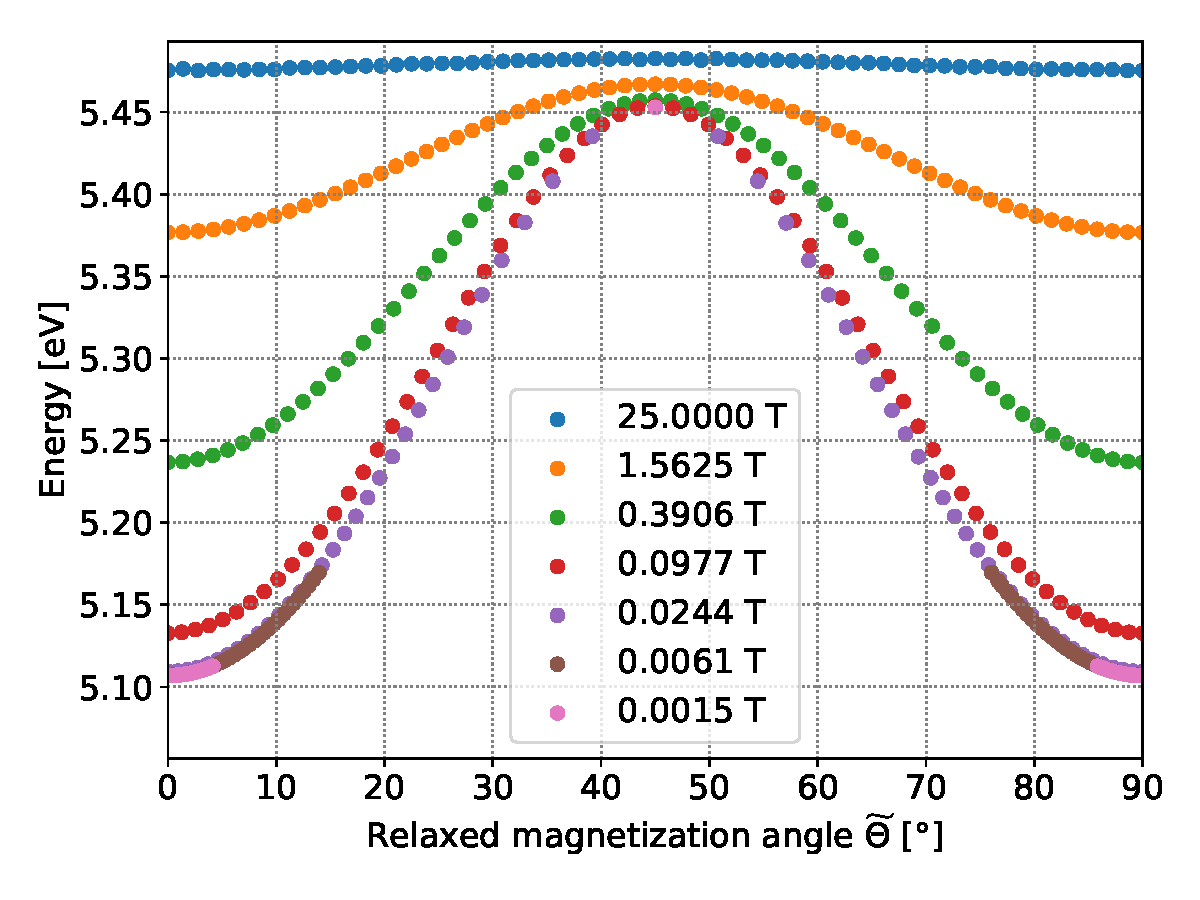
\includegraphics[width=0.9\columnwidth]{Figures/Plus_65_B25-0.001-div4_a128Pi_plotOptimized.pdf}
    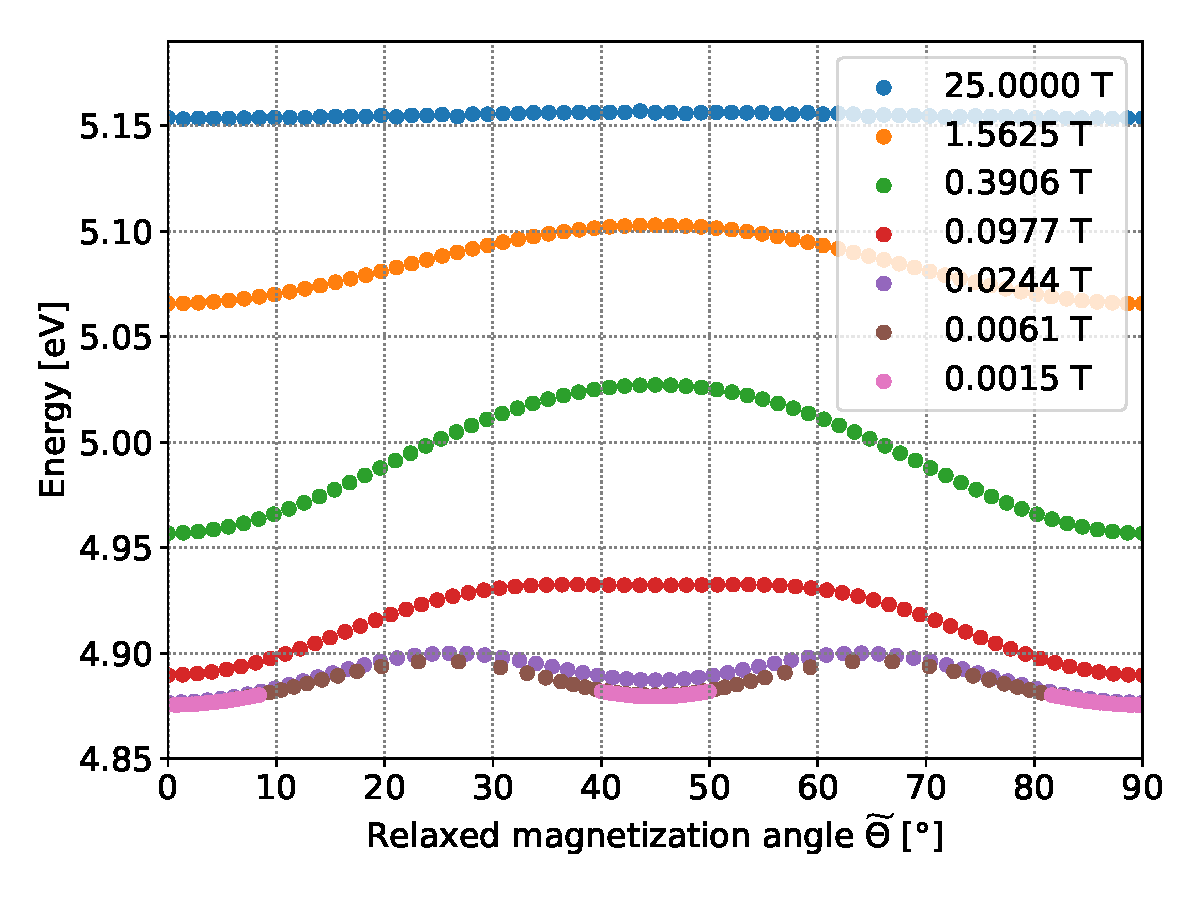
\includegraphics[width=0.9\columnwidth]{Figures/Plus_48.2_B25-0.001-div4_a128Pi_plotOptimized.pdf}
    \caption{Energy landscape for various probing field magnitudes, as listed in the legend. $\widetilde{\chi}$ is varied uniformly in 64 steps from \SI{0}{\degree} to \SI{90}{\degree}. The horizontal axis denotes the average magnetization angle $\widetilde{\Theta}$ after relaxation. \textbf{Top:} $\rho=0.65$. \textbf{Bottom:} $\rho=0.49$.}
    \label{fig:EA_EnergyLandscape}
\end{figure}
All of $E(\widetilde{\Theta}~=~n\SI{45}{\degree}), n\in\mathbb{Z}$ are equilibria, due to the symmetry of the geometry. Of these, 4 are energy minima, and 4 are maxima. The energy difference between these minima and maxima is the \textit{energy barrier} between stable states. To determine the energy barrier, the energy landscape $E(\widetilde{\Theta})$ is calculated. For an accurate calculation, one has to allow the magnetization to relax, i.e. to settle itself to the geometry. This is mainly because, for a perfectly uniform magnetization, all magnetization angles have equal energy, resulting in a flat energy landscape, from which the energy barrier can not be determined. To prevent the magnetization from relaxing all the way to an anisotropic energy minimum, a probing field is applied at the desired angle. The Zeeman energy term due to the probing field is then subtracted, to reveal the energy landscape of a single biaxial island. This energy landscape is shown for $\rho=0.65$ in \cref{fig:EA_EnergyLandscape} (top), for various probing field magnitudes. For very high magnitudes, the energy landscape is nearly flat, because for such high fields the magnetization is nearly uniform. The relaxation towards the energy minimum (which the probing field should prevent) is clearest for low field magnitudes. Note that, even for very small fields, the energy maximum at $\widetilde{\Theta} = \SI{45}{\degree}$ is stable, such that the probing field is not strictly necessary if one is only interested in the energy barrier, rather than the whole energy landscape. \par
\begin{figure}
    \centering
    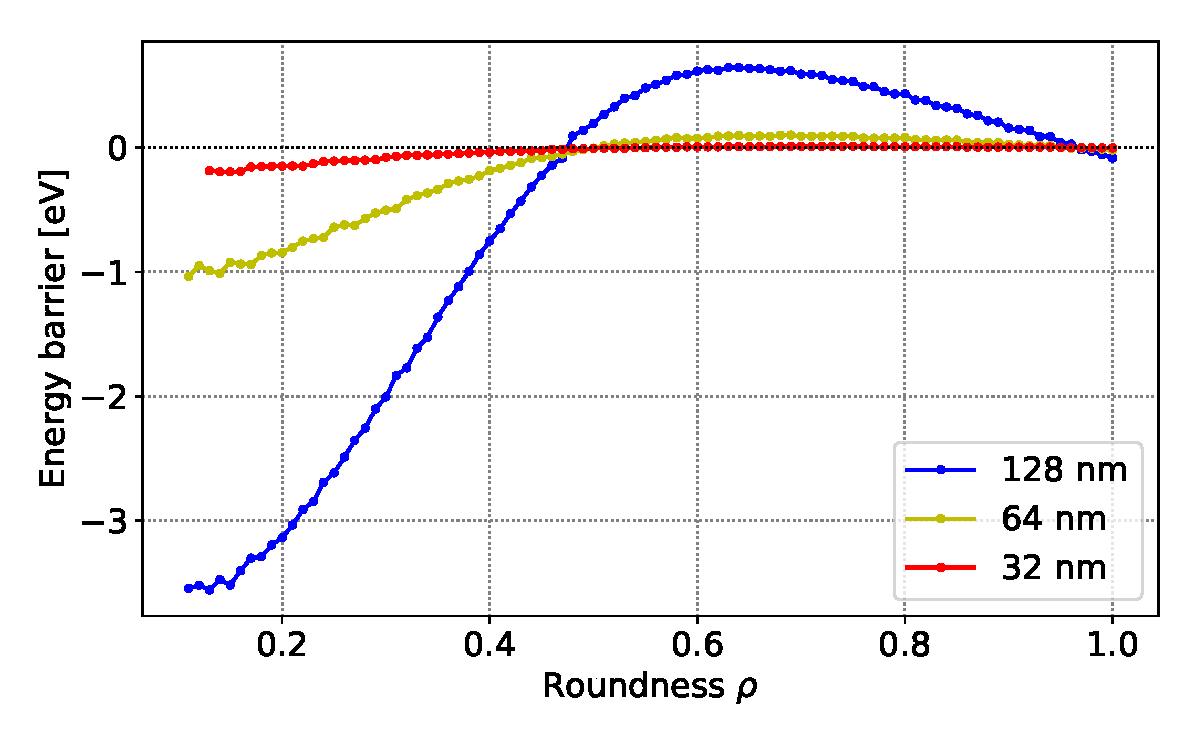
\includegraphics[width=0.9\columnwidth]{Figures/Plus_32,64,128_0.1-1_aPi128_B0.01_cell1nm.pdf}
    \caption{Energy barrier as a function of roundness $\rho$, for different total sizes $L$ as listed in the legend. A positive value indicates that $E(\Theta=\SI{45}{\degree}) > E(\Theta=\SI{0}{\degree})$, i.e. the hard axes are diagonal.}
    \label{fig:EA_EnergyRoundnessDependence}
\end{figure}
\begin{figure}
     \centering
     \hskip2em
         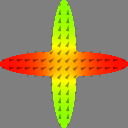
\includegraphics[width=0.3\columnwidth]{Figures/biaxial_island/BarrierMagnetization/mPlus_roundness0.20_a0.79.png}
     \hskip2em
         
\includegraphics[width=0.3\columnwidth]{Figures/biaxial_island/BarrierMagnetization/mPlus_roundness0.60_a0.00.png}
    \caption{Relaxed magnetization for two different geometries with $L=\SI{100}{\nano\metre}$. The color hue represents the in-plane magnetization angle. \textbf{Right:} $\rho=0.2$. \textbf{Left:} $\rho=0.6$.}
    \label{fig:EA_EnergyMagnetization}
\end{figure}
The energy barrier $E_{\mathrm{barrier}}$ strongly depends on the roundness, as shown in \cref{fig:EA_EnergyRoundnessDependence}. It is observed that, for large $\rho$, the easy axes are the long axes of the ellipses, while the hard axes are the diagonals in between them. For $\rho < 0.48$, the opposite is true. This is understood by looking at the detailed magnetization profile for both large and small $\rho$, shown in \cref{fig:EA_EnergyMagnetization}. For small $\rho$, the geometry consists of four elongated arms. In each of these arms, the magnetization prefers to be aligned along the length of that arm. The combination of those horizontal and vertical magnetizations, with a domain wall in the center, is on average diagonal, such that it appears as if the easy axes are diagonal. This is no longer a single-domain nanomagnet, so care must be taken when using low-$\rho$ islands, as the magnetization can differ significantly between the arms. \par
In between the regimes of small and large $\rho$, the energy barrier is very low, and for $\rho\approx 0.49$ the energy difference $\Delta E_{\SI{45}{\degree}-\SI{0}{\degree}}=E(\Theta=\SI{45}{\degree})-E(\Theta=\SI{0}{\degree})$ becomes zero. The energy landscape for $\rho=0.49$ is shown in \cref{fig:EA_EnergyLandscape} (bottom). Even though $\Delta E_{\SI{45}{\degree}-\SI{0}{\degree}}=0$, the energy landscape is not entirely flat. Instead, there are now 8 local minima instead of 4, with a low energy barrier in between them all.

\subsection{Thermal switching}
At nonzero temperatures, random thermal fluctuations can allow the magnetization to overcome the energy barrier and switch between stable states. Due to the thermal nature of this process, the magnetization reorientation rate is assumed to follow an Arrhenius form~\cite{FAR-13}. The thermal switching can then be modeled as driven by a jump-noise process~\cite{MagDynamics_JumpNoise}. As such, in the regime where $E_{\mathrm{barrier}} \gg k_B T$, the time $t_i$ between two consecutive switches is given by
\begin{equation}
    t_i = -\frac{1}{f_0}\exp(\frac{E_{\mathrm{barrier}}}{k_B T}) \ln(1-P_i) \mathrm{,}
    \label{eq:EA_Switching_t_i}
\end{equation}
with $P_i$ a uniformly distributed random number between 0 and 1. A theoretical equation~\cite{MuMax3,LEL-17b,f0_mumax3_reference} for $f_0$ (in \si{\radian\per\second}) is given by
\begin{equation}
    f_0 = \gamma \frac{\alpha}{1+\alpha^2} \frac{2}{M_{\mathrm{sat}} V} \sqrt{\frac{E_{\mathrm{barrier}}^3}{\pi k_B T}} \mathrm{,}
    \label{eq:EA_Switching_theoretical}
\end{equation}
with $\gamma$ the gyromagnetic ratio, $M_{\mathrm{sat}}$ the saturation magnetization, and $\alpha$ the damping constant.
For a biaxial island with $E_{\mathrm{barrier}}=\SI{154.7}{\milli\electronvolt}$, volume $V\approx\SI{4e-23}{\metre\cubed}$, $M_{\mathrm{sat}}=\SI{8e5}{\ampere\per\metre}$ and $\alpha=0.01$, at $T=\SI{300}{\kelvin}$, this yields $f_0=\SI{6e5}{\per\second}$. \par
One can also estimate $f_0$ by rewriting \cref{eq:EA_Switching_t_i}, given $N$ switches during a time interval $\tau$:
\begin{equation}
    f_0 = \frac{N \ln(4)}{\tau} \exp(\frac{E_{\mathrm{barrier}}}{k_B T}) \mathrm{.}
\end{equation}
Simulations were carried out for various temperatures and energy barriers, the results of which are given in \cref{tab:Switching_f0}. The values for $N$ were obtained by counting every monotone rotation of the magnetization over an angle greater than \SI{90}{\degree} as a single switch.
\ctable[
    cap = Switching Rates,
    caption = {Values of the attempt frequency $f_0$ for different energy barriers and temperatures. $M_{\mathrm{sat}}=\SI{8e5}{\ampere\per\metre}$ and $\alpha=0.01$ for all entries.},
    label = {tab:Switching_f0},
    pos = t!,
    %sideways
    ]{
    c|c|c|c||c
    }{
    \tnote[a]{This energy barrier is comparable to the thermal energy $k_B T$. Hence, the switching rate ($\approx \SI{2}{\nano\second}$) is on the same timescale as the LLG dynamics, which causes the estimate for $f_0$ using \cref{eq:EA_Switching_theoretical} to be inaccurate.}
    }{
        Barrier [\si{\milli\electronvolt}] & T [\si{\kelvin}] & $\tau$ [\si{\nano\second}] & $N$ & $f_0$ [\si{\per\second}] \\
        \hline
        27.8\tmark[a] & 300 & 100 & 37 & \SI{1.50e9}{} \\
        \hline
        154.7 & 273 & 1000 & 13 & \SI{1.29e10}{} \\
        154.7 & 300 & 1000 & 11 & \SI{6.05e9}{} \\
        154.7 & 350 & 1000 & 41 & \SI{9.60e9}{} \\
        207.9 & 350 & 1000 & 9 & \SI{1.23e10}{} \\
        240.7 & 350 & 1000 & 5 & \SI{2.03e10}{} 
    }
These values are on the order of $f_0=\SI{e10}{\per\second}$, which does not agree with the theoretical value. It is hypothesized that this is because the magnetization of the islands is not perfectly uniform, which is one of the assumptions underlying the theoretical equation. The values obtained through simulations are, however, on the same order of magnitude as the resonance frequency of the magnetization in a local energy minimum of the energy landscape from \cref{fig:EA_EnergyLandscape}. The oscillation in this energy minimum can be interpreted as an attempt to switch to another stable state, once every half-period.

\section{Half adder}
\begin{figure*}[ht!]
    \centering
    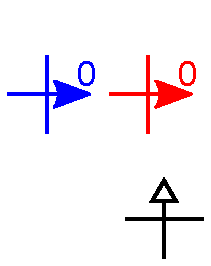
\includegraphics[width=0.16\textwidth]{Figures/HalfAdderConcept/Input 0 deg arrowtext.pdf}
    \rulesep
    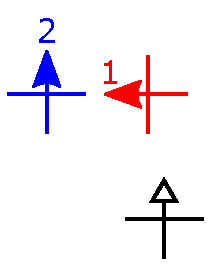
\includegraphics[width=0.16\textwidth]{Figures/HalfAdderConcept/Input 90 deg arrowtext.pdf}
    \rulesep
    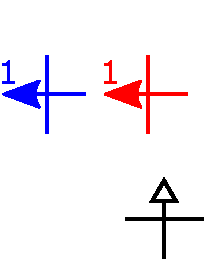
\includegraphics[width=0.16\textwidth]{Figures/HalfAdderConcept/Input 180 deg arrowtext.pdf}
    \rulesep
    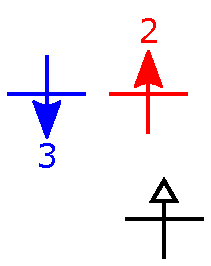
\includegraphics[width=0.16\textwidth]{Figures/HalfAdderConcept/Input 270 deg arrowtext.pdf}
    \hskip4em
    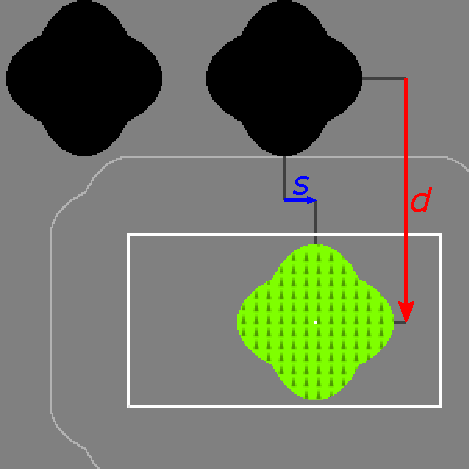
\includegraphics[width=0.2\textwidth]{Figures/regions000006.pdf}
    \caption{\textbf{Left:} lowest energy configurations for all four possible input magnetizations. This functions as a half adder with quaternary convention $(0,2,1,3)$. Islands with a filled arrowhead can move their magnetization freely to achieve the lowest energy. Islands with an open arrowhead have their magnetization permanently fixed in the direction of the arrow. The blue island is the input island, the red island functions as the output. \textbf{Right:} geometry to scale, defining the quantities $s$ and $d$. The white rectangle indicates the range in \cref{fig:EA_HalfAdderRegions1}.}
    \label{fig:EA_HalfAdderConcept1}
\end{figure*}
\ctable[
    cap = Half Adder,
    caption = {Truth table for a half adder, both in binary and quaternary numeral systems.},
    label = {tab:HalfAdder},
    pos = b!,
    mincapwidth = 0.7\columnwidth
    ]{
    c|c||c|c % paps vindt dit beter
    }{}{
        \multicolumn{2}{c||}{Binary} & \multicolumn{2}{c}{Quaternary} \\
        \hline
        Input & Output & Input & Output \\
        \hline
        00 & 00 & 0 & 0 \\
        01 & 01 & 1 & 1 \\
        10 & 01 & 2 & 1 \\
        11 & 10 & 3 & 2 \\
    }
A half adder is a logic gate which adds two binary input bits, and therefore yields two bits as
output. The truth table of a binary half adder is given in the left half of \cref{tab:HalfAdder}. Since both input and output are represented by two bits, they can also each be represented by a biaxial island, because a single biaxial island has 4 stable states and can thus represent exactly two bits of information. As such, a half adder realized with biaxial nanomagnets only has one input island and one output island. The truth table of a half adder represented in the quaternary numeral system inherent to biaxial nanomagnets is given in the right half of \cref{tab:HalfAdder}.
\subsection{Nanomagnetic half adders}
When designing a nanomagnetic logic gate, one has to define the meaning of each stable magnetization direction. For biaxial nanomagnets, there are four such directions, which have to be assigned a number from 0 to 3. There are 24 possible ways to do this. We will refer to such a choice as the `\textit{quaternary convention}', and will always list the quaternary convention in the form $(\SI{0}{\degree}, \SI{90}{\degree}, \SI{180}{\degree}, \SI{270}{\degree})$, for the island geometry from \cref{fig:EA_geom}. A given geometry of nanomagnets, with given input and output islands, will only behave as a half adder for at most one quaternary convention. When choosing a different input or output island, the relevant quaternary convention may be different, or nonexistent. Thus, given a geometry with $N$ free islands, one can try $N$ choices for the input island, $N-1$ for the output, and 24 possible quaternary conventions (if one uses the same convention for input and output). Only a select few, if any, of these $24N(N-1)$ choices will correctly give the geometry the meaning of a half adder. \par
A given geometry can work as a half adder in a forward calculation if there exists such a choice where, for each of the 4 possible input magnetization angles, the lowest energy state has the logically correct output magnetization angle. \par
Also, note that in any NML system it is necessary to include at least one island whose magnetization direction is permanently fixed, in order to break the symmetry. This is because a nanomagnetic system is invariant under a global magnetization reversal~\cite{GYP-18}. Such fixation can for example be realized using exchange bias~\cite{ExchangeBias,ExchangeBias_nanostructures,ExchangeBias_Mechanisms}.

\subsection{Gate design}
A schematic representation of the half adder proposed here is shown in \cref{fig:EA_HalfAdderConcept1}, where the ground states for all four possible input magnetization directions are shown. The reasoning behind this geometry is as follows. \par
From the truth table of the half adder, it can be noted that there must be two inputs for which input and output are equal: $0\rightarrow0$ and $1\rightarrow1$. This condition is readily fulfilled for two biaxial islands aligned along their easy axes in a `++' geometry. The lowest energy state of such a geometry has both islands with a parallel magnetization along their common axis ($\rightarrow \rightarrow$ or $\leftarrow \leftarrow$). The anti-parallel configuration perpendicular to the common axis ($\uparrow~\downarrow$ or $\downarrow~\uparrow$) is another equilibrium with slightly higher energy, and is stable if the islands have a nonzero energy barrier. \par
As such, two of the four inputs are already mapped to a correct output, if one identifies the horizontal directions with $0$ and $1$ in the quaternary convention. Also $3\rightarrow2$ is fulfilled, as this corresponds to the anti-parallel configuration if one identifies the vertical directions with $2$ and $3$. The only rule which is not yet fulfilled is $2\rightarrow1$, which then requires a vertical input to be mapped to a horizontal output. This can be fulfilled by adding a permanently fixed island, in the manner shown in \cref{fig:EA_HalfAdderConcept1}, with its magnetization pointing towards the output island. Hence, this fixed island prevents the output island magnetization from pointing toward the fixed island. Hence, if one identifies the `up' direction with the quaternary number 2, the output will have horizontal magnetization, and this horizontal direction is then identified with the number 1. \par
In order to assess the balancedness of the half adder, two metrics are introduced: $B_1 = \min_\alpha(E_{\alpha,1}) - \max_\alpha(E_{\alpha,0})$ and $B_2 = \max_\alpha(E_{\alpha,0}) - \min_\alpha(E_{\alpha,0})$. Here, $E_{\alpha,i}$ represents the $i$-th lowest energy level for which the input magnetization angle is near $\alpha$. The four ground states corresponding to the four possible inputs are hence represented by $E_{\alpha,0}$. The first metric $B_1$ represents the energy difference between the highest ground state and the lowest first excited state. If the gate is to be used in a reverse calculation, $B_1$ should at least be positive, because then, in thermal operation, the correct states will occur with higher probability than the incorrect states. The second metric $B_2$ gives the energy difference between the highest and lowest of the 4 ground states, and is exactly zero for a perfectly balanced gate. If it is nonzero, one of the ground states is lower in energy than another, such that there is a chance that this particular logical state will be favored when multiple half adders are put in series. Hence, for a large forward calculation, $B_2$ is preferably as small as possible. \par

\subsection{Varying fixed island position}
We will now vary the position of the fixed island, to improve the values of $B_1$ and $B_2$. This position is determined by the parameters $s$ ad $d$, as defined in the rightmost part of \cref{fig:EA_HalfAdderConcept1}, where the range over which they were varied is represented by the white rectangle. The results of varying these parameters are shown in \cref{fig:EA_HalfAdderRegions1}.
\begin{figure}
    \centering
    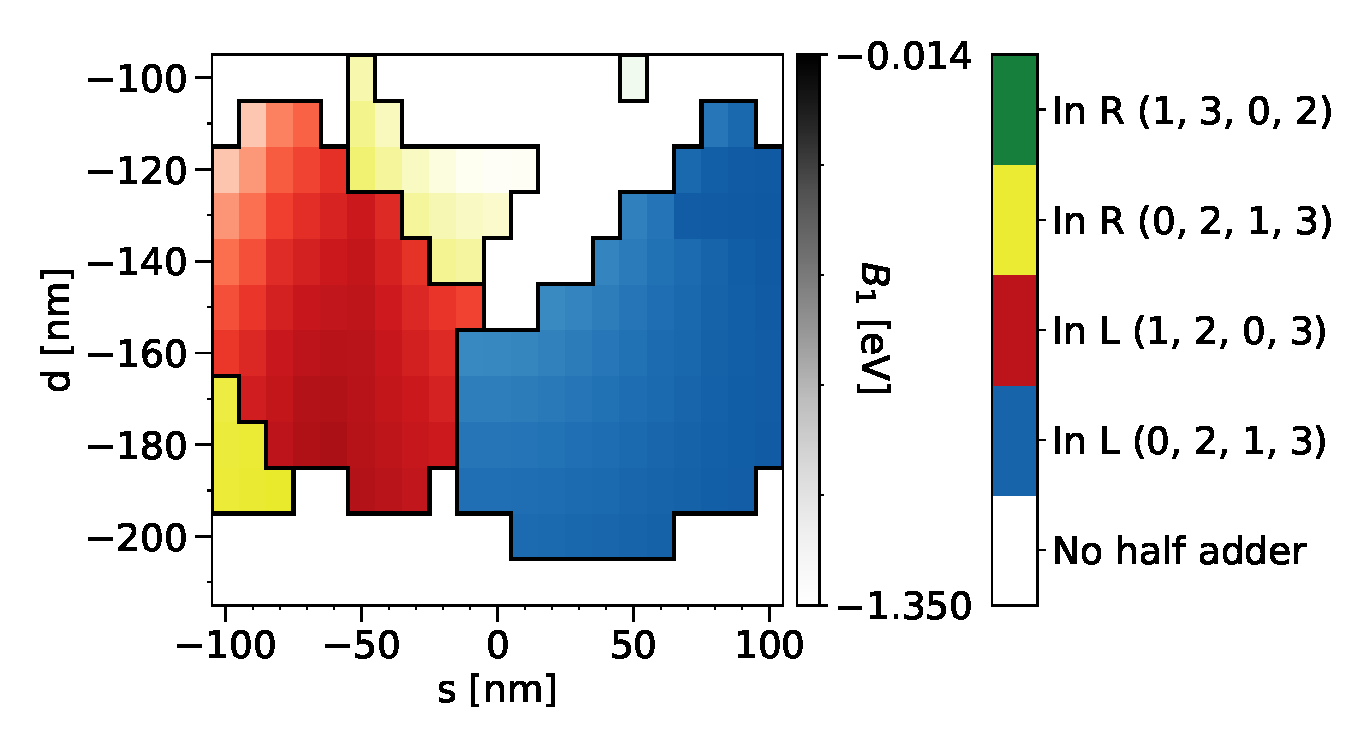
\includegraphics[width=\columnwidth]{Figures/table(d100-210_10,s-100-100_10)_balanced1.pdf}
    \vskip0em
    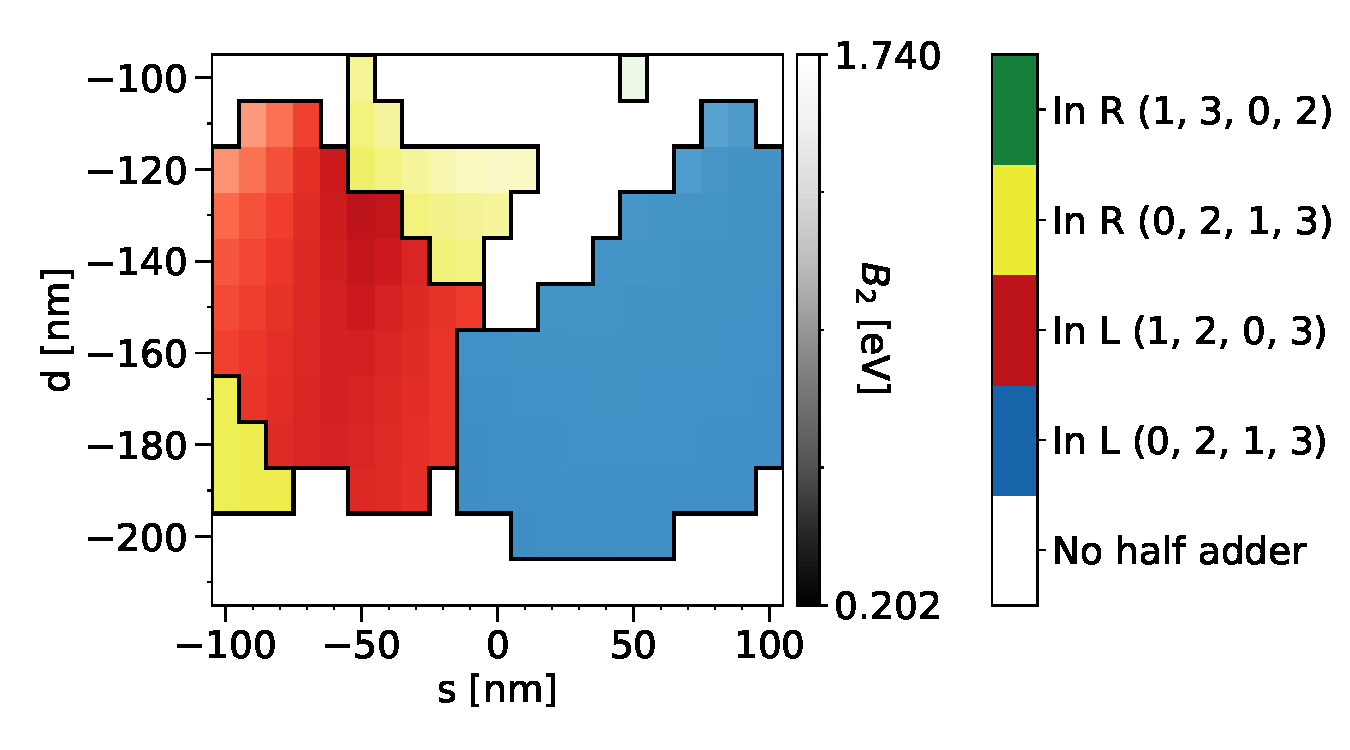
\includegraphics[width=\columnwidth]{Figures/table(d100-210_10,s-100-100_10)_balanced2.pdf}
    \caption{Regions where the geometry functions as a half adder, according to the quaternary convention indicated by the color. The brightness represents the balancedness metrics (darker is better). `In L' or `In R' indicate that the input is the leftmost or rightmost free island, respectively.}
    \label{fig:EA_HalfAdderRegions1}
\end{figure}
It is observed that there are several regions where the geometry can be interpreted as a half adder. This interpretation is given by the quaternary convention, as indicated by the color. The brightness of these colors represents the balancedness metrics. In the blue region, the geometry functions as initially conceived, as was shown schematically in \cref{fig:EA_HalfAdderConcept1}. The red and yellow regions overlap, because the yellow region is the mirrored counterpart of the red region over the $s=\SI{-64}{\nano\metre}$ axis. Unfortunately, the first metric $B_1$ is negative everywhere in this range of $s$ and $d$, preventing a reverse calculation. An example of the energy levels, grouped by input, is shown in \cref{fig:EA_HalfAdderLevels1} for $d=\SI{-170}{\nano\metre}$ and $s=\SI{-60}{\nano\metre}$, which has one of the best, i.e. least negative, values for $B_1$ in the examined range. \par
\begin{figure}
    \centering
    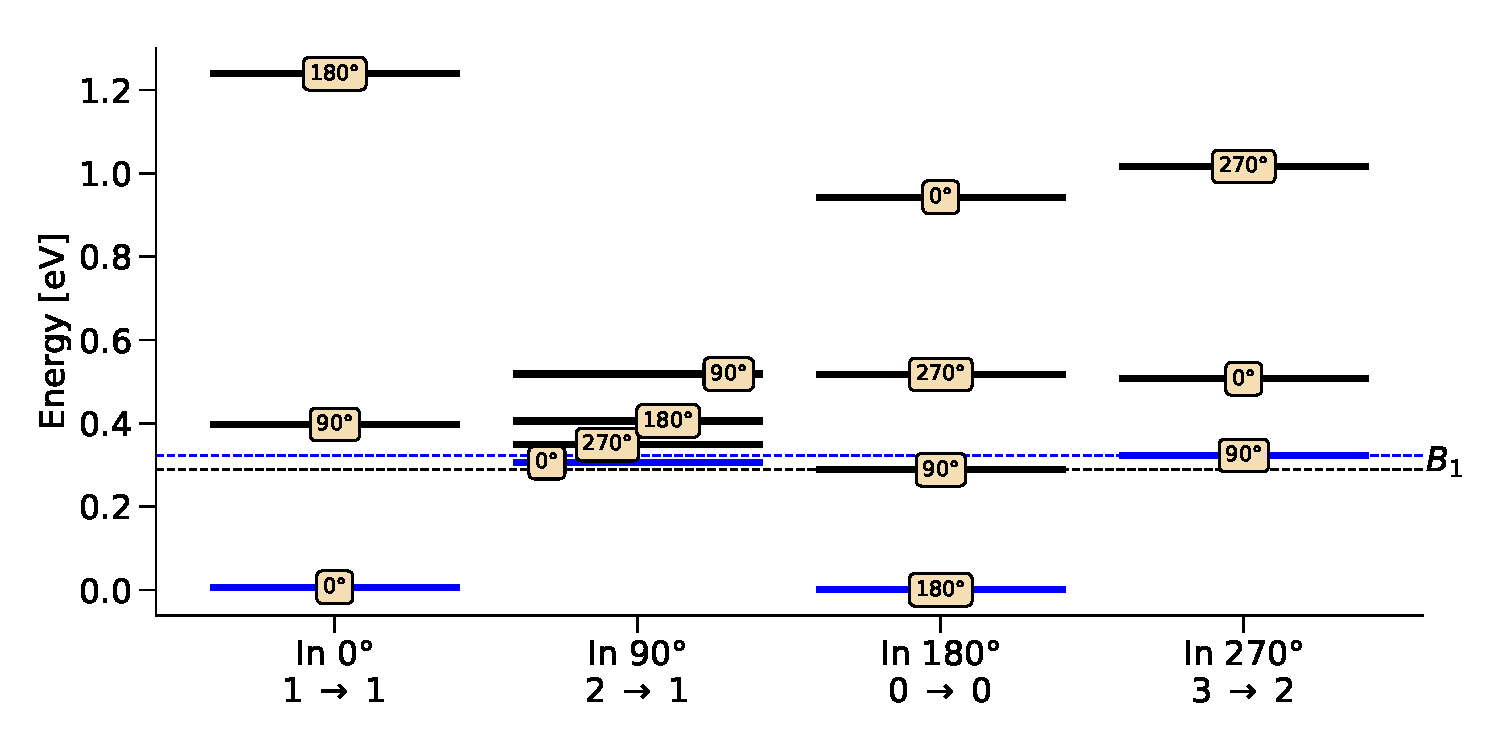
\includegraphics[width=\columnwidth]{Figures/table(d170,s-60)_energylevels.pdf}
    \caption{Energies of different magnetization configurations, grouped by input magnetization angle, for $d=\SI{-170}{\nano\metre}$ and $s=\SI{-60}{\nano\metre}$. Blue states are logically correct. The text box on each energy level shows the output magnetization angle for that state.}
    \label{fig:EA_HalfAdderLevels1}
\end{figure}
\begin{figure}
    \centering
    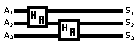
\includegraphics[width=0.5\columnwidth]{Figures/Layout_halfadderchain_annotated.pdf}
    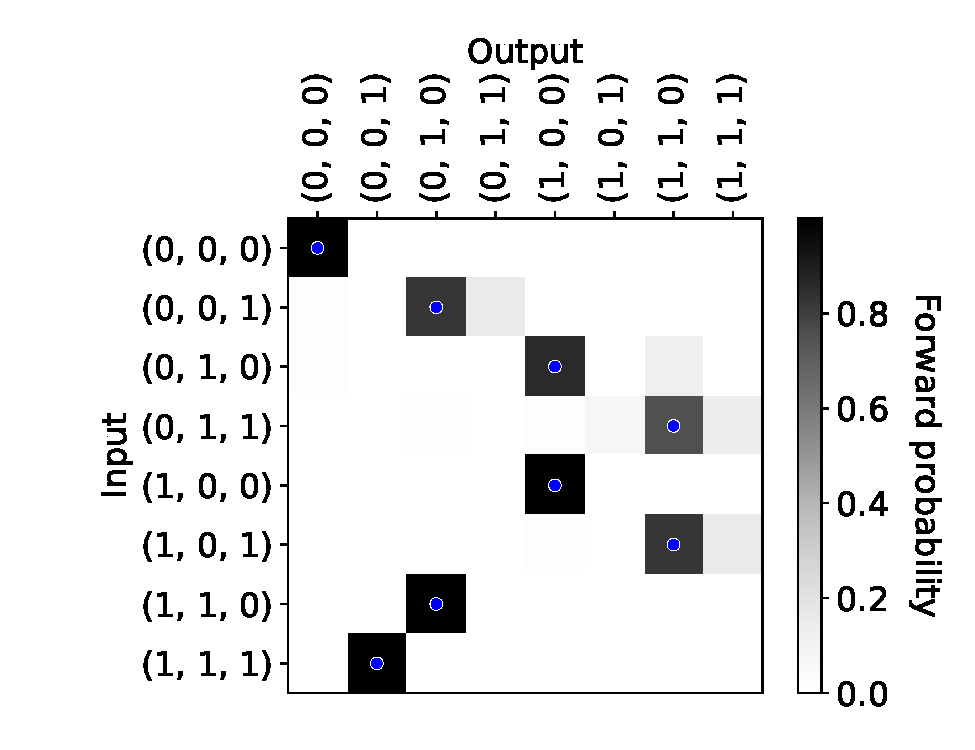
\includegraphics[width=0.8\columnwidth]{Figures/table(d170,s-60)_forward1_probabilities_T0.0258eV.pdf}
    \caption{\textbf{Top:} schematic representation of the logic circuit. \textbf{Bottom:}
    probability of each output, when fixing the input (i.e. forward calculation), at \SI{298}{\kelvin}. Hence, each row adds up to a total of 1. Blue dots indicate the correct output. Inputs are in $(A_1, A_2, A_3)$ format, outputs $(S_1, S_2, S_3)$.}
    \label{fig:EA_HalfAdderCircuit1}
\end{figure}
The second metric shows how well-suited a certain choice of $s$ and $d$ is for forward calculation. $B_2$ does not become exactly zero for this type of geometry. As such, only a limited number of half adders can be placed in a forward-calculating circuit. \par
An example of such a circuit is shown in \cref{fig:EA_HalfAdderCircuit1} (top), where the half adders are represented in binary form. The bottom part of \cref{fig:EA_HalfAdderCircuit1} shows the probability of each output for a forward calculation, i.e. when fixing the global input $A_1$, $A_2$ and $A_3$, at room temperature (\SI{298}{\kelvin}). It is observed that the logically correct output states are the most likely to occur. Some incorrect states also have nonzero probability, which can be explained with the energy levels from \cref{fig:EA_HalfAdderLevels1}. For example, the energies for input 10 (quaternary 2) are closely spaced, which in this circuit is the main cause of incorrect results with nonzero probability.
An issue for larger circuits, is that the ground states for inputs 1 and 0 have significantly lower energy than for inputs 2 and 3. As such, it can be energetically favorable for a half adder inside a circuit to have input 1 or 0, which can yield incorrect results with appreciable probability. \par
There also exists a different range for $s$ and $d$ where $B_1$ is positive, hence allowing at least one reverse calculation. This range has the fixed island closer to the common axis of the free islands, around $(s,d) = (\SI{130}{\nano\metre}, \SI{-50}{\nano\metre})$. Unfortunately, the values of $B_2$ in this range are higher, thus making half adders in this range less suitable for forward calculation. Because in this case the fixed island is closer to the output island, it can also be more difficult to connect nanomagnetic wires to the input and output without significantly disturbing the system.

\section{Conclusion}
Before considering half adders, the energy landscape of a single biaxial island was examined. It was found that relaxation is necessary for anisotropy to occur: if the island has a perfectly uniform in-plane magnetization, the energy is equal for any of these magnetization directions. The energy barrier significantly depends on the roundness $\rho$ of the ellipses constituting the biaxial island. For large $\rho$, the easy axes are equal to the long axes of these ellipses. For small $\rho$, the easy and hard axes appear to be swapped, because the geometry more clearly consists of four perpendicular arms, which on average yield a diagonal magnetization. At $\rho \approx 0.49$, the energy difference between an average magnetization angle of \SI{0}{\degree} and \SI{45}{\degree} becomes zero. However, the energy landscape is not entirely flat; due to the relaxation along the edges of the geometry, there are 8 stable states instead of 4. \par
The thermal switching of different biaxial islands and for different temperatures and damping constants was also examined. No agreement between theoretical and simulated values for the attempt frequency $f_0$ was found. It was hypothesized that this is because the magnetization of the islands is not perfectly uniform, which is one of the assumptions underlying the theory. The value obtained through simulations is approximately $f_0=\SI{e10}{\per\second}$, which is on the same order of magnitude as the intrinsic resonance frequency of the magnetization in the local minima of the energy landscape. \par
Two similar half adder geometries were proposed, which can perform a forward calculation. One of these geometries has the fixed island far from the common axis, while for the second geometry the fixed island was placed near the common axis. The first geometry is more suitable for forward calculation, because its ground state energies are closer together than for the second geometry. Unfortunately, it is not perfectly balanced, so the size of a forward calculating circuit is limited. Only the second geometry can under ideal circumstances be used for a single reverse calculation, since all of its logically incorrect states have higher energy than any of the correct states.

% TODO: check if the references are decently formatted, because this bibliography style shows a lot more

\nocite{*}
\bibliographystyle{phdsymp}
\bibliography{smallbibliography}

\end{document}
